\begin{center}
\LARGE
Matematikscreening 
\end{center}
\stepcounter{section}



\begin{opgavetekst}{Opgave 1}
	En lineær funktion $f$ er givet ved
	\begin{align*}
		f(x) = 3x-12,
	\end{align*}
\end{opgavetekst}
\begin{delopgave}{(5 point)}{1}
	Aflæs hældningen for $f$ samt skæringen med $y$-aksen for $f$. 
\end{delopgave}
\begin{delopgave}{(5 point)}{2}
	Bestem $f(4)$.
\end{delopgave}

\begin{opgavetekst}{Opgave 2}
	En ligning er givet ved
	\begin{align*}
		-7x+14 = 4x-17.
	\end{align*}
\end{opgavetekst}
\begin{delopgave}{(10 point)}{1}
	Løs ligningen \textbf{uden} brug af \textit{solve}, hvor du argumenter for, hvad du gør linje for linje.
\end{delopgave}
\begin{delopgave}{(5 point)}{2}
	Løs ligningen \textbf{med} brug af \textit{solve}, og undersøg om dit resultat passer med resultatet fra i).
\end{delopgave}



\begin{opgavetekst}{Opgave 3}
	På Fig. \ref{fig:lines3} ses graferne for tre lineære funktioner $f$, $g$ og $h$ med forskrifterne 
	\begin{align*}
		f(x) &= 2x-1,\\
		g(x) &= x+1,\\
		h(x) &= -x+2.
	\end{align*}
	Desuden ses punktet $P(1,y)$, der ligger på skæringen mellem graferne $A$ og $C$.
	\begin{figure}[H]
		\centering
		\begin{tikzpicture}
			\begin{axis}[
				axis lines = center,
				xmin = -3,
				ymin = -1
				]
				\addplot[samples = 10, color = green] {x+1};
				\addplot[samples = 10, color = red]	{2*x-1};
				\addplot[samples = 10, color = blue] {-x+2};
				\node[circle, fill = purple, inner sep = 0pt, minimum size = 5pt] at (axis cs: 1,1) {};
				\node at (axis cs:1.4,1) {$P$};
				\draw[dashed, color = gray, thick] (axis cs: 1,0 ) -- (axis cs:1,1);
				\draw[dashed, color = gray, thick] (axis cs: 0,1 ) -- (axis cs:1,1);
				\node at (axis cs:-0.3,1) {$y$};
				\node[color = blue] at (axis cs:-0.9,3.5) {$A$};
				\node[color = green] at (axis cs:4,5.5) {$B$};
				\node[color = red] at (axis cs:3,6) {$C$};
			\end{axis}
			\node at (9,0.7) {(1)};
			\node at (3.15,7.5) {(2)};
		\end{tikzpicture}
		\caption{Graferne for funktionerne $f$, $g$ og $h$.}
		\label{fig:lines3}
	\end{figure}\phantom{h}
\end{opgavetekst}
\begin{delopgave}{(10 point)}{1}
	Afgør, hvilke af graferne $A$, $B$ og $C$, der tilhører funktionerne $f$, $g$ og $h$. 
\end{delopgave}
\begin{delopgave}{(5 point)}{2}
	Bestem andenkoordinaten $y$ i punktet $P(2,y)$ på Fig. \ref{fig:lines3}.
\end{delopgave}

\begin{opgavetekst}{Opgave 4}
	På Fig. \ref{fig:oneline3} ses grafen for en lineær funktion $f$ givet ved
	\begin{align*}
		f(x) = ax + b
	\end{align*}
	samt grafen for en lineær funktion $g$.
	\begin{figure}[H]
		\centering
		\begin{tikzpicture}
			\begin{axis}[
				axis lines = center,
				xmin = -1,
				ymin = -5, 
				xmajorticks=false,
				ytick = {-3}
				]
				\addplot[samples = 10, color = blue!40, thick] {-x+6};
				\addplot[samples = 10, color = red!40, thick] {2*x-3};
				\node[circle, fill = purple, inner sep = 0pt, minimum size = 5pt] at (axis cs: 1,5) {};
				\node[circle, fill = purple, inner sep = 0pt, minimum size = 5pt] at (axis cs: 3,3) {};
				\node at (axis cs:1.7,5) {$P(1,5)$};
				\node at (axis cs:3.7,3) {$Q(3,3)$};
				\node at (axis cs:4,1) {$\color{blue!60} f$};
				\node at (axis cs:4,6) {$\color{red!60} g$};
			\end{axis}
			\node at (8.9,3.0) {(1)};
			\node at (1.4,7.5) {(2)};
		\end{tikzpicture}
		\caption{Graferne for $f$ og $g$.}
		\label{fig:oneline3}
	\end{figure}\phantom{h}
\end{opgavetekst}
\begin{delopgave}{(10 point)}{1}
	Brug punkterne $P$ og $Q$ på Fig. \ref{fig:oneline3} til at bestemme $a$ og $b$. 
\end{delopgave}
\begin{delopgave}{5 point)}{2}
	Bestem skæringen med $y$-aksen for $g$. 
\end{delopgave}
\begin{delopgave}{(5 point)}{3}
	Brug dit svar på ii) samt at $g(3) = 3$ til at bestemme en forskrift for $g$.
\end{delopgave}

\begin{opgavetekst}{Opgave 5}
	\begin{center}
		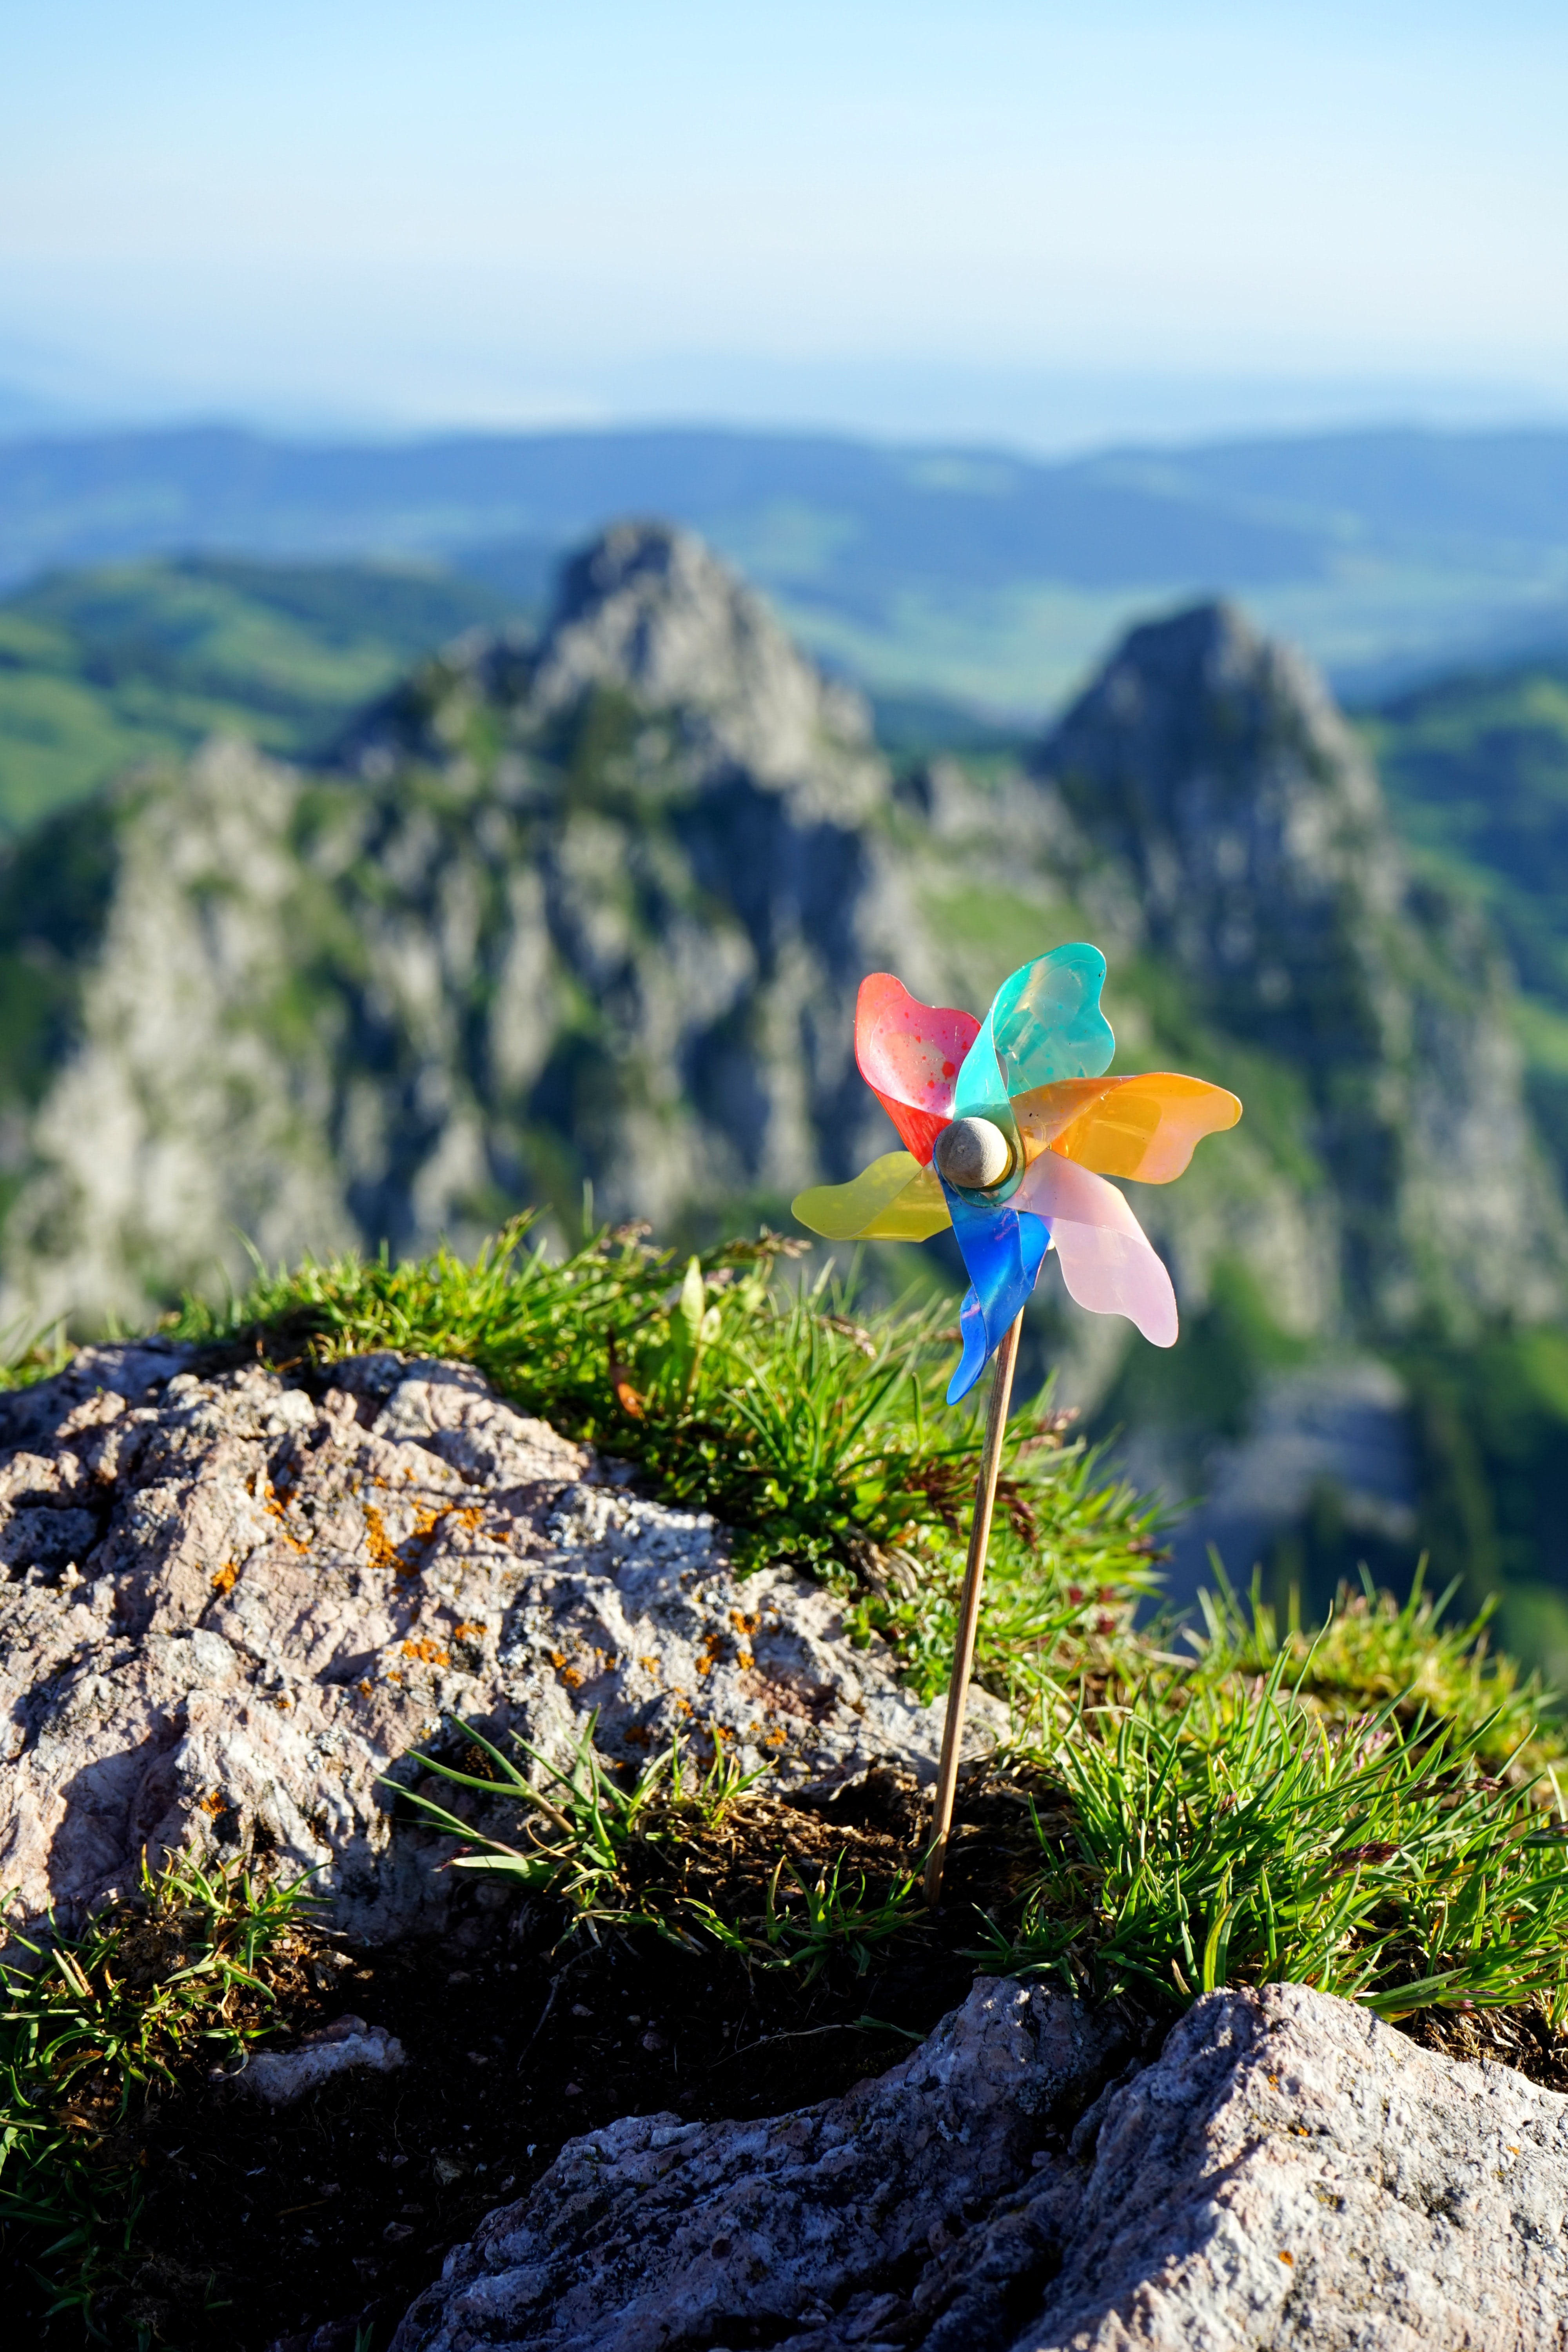
\includegraphics[width=0.4\textwidth]{Billeder/windmill.jpg}
	\end{center}
	Grundet høje energipriser installerer en familie en lille vindmølle på deres gård. De måler effekten (i Watt) af deres vindmølle som funktion af vindhastigheden 
	(i meter pr. sekund) og samler deres 
	målinger. Disse kan ses i Tab. \ref{tab:vind}.
	\begin{table}[H]
		\centering
		\begin{tabular}{c|c|c|c|c|c}
			Vindhastighed (m/s) & 1 & 3 & 4 & 7 & 10 \\
			\hline
			Effekt (W) & 201 & 604 & 789 & 1368 & 1991 
		\end{tabular}
		\caption{Effekt af vindmølle.}
		\label{tab:vind}
	\end{table}
	Vi antager, at effekten af netop denne type vindmølle kan beskrives ved en sammenhæng af typen
	\begin{align*}
		P(x) = ax+b,
	\end{align*}
	hvor $P$ er effekten af vindmøllen (i Watt) og $x$ er vindhastigheden (i meter pr. sekund).
\end{opgavetekst}
\begin{delopgave}{(10 point)}{1}
	Brug tallene fra Tab. \ref{tab:vind} til at bestemme $a$ og $b$. 
\end{delopgave}
\begin{delopgave}{(5 point)}{2}
	Forklar, hvad tallet $a$ betyder for modellen. 
\end{delopgave}
\begin{delopgave}{(10 point)}{3}
	Brug modellen til at afgøre, hvad effekten af vindmøllen er, hvis det blæser med en vindhastighed på 12 m/s.
\end{delopgave}

\begin{opgavetekst}{Opgave 6}
	To funktioner $f$ og $g$ har forskrifterne 
	\begin{align*}
		f(x) &= 5x-4, \\
		g(x) &= -2x+10.
	\end{align*}
\end{opgavetekst}
\begin{delopgave}{(5 point)}{1}
	Bestem skæringspunktet mellem grafen for $g$ og $x$-aksen.
\end{delopgave}
\begin{delopgave}{(10 point)}{2}
	Bestem skæringspunktet mellem graferne for $f$ og $g$. 
\end{delopgave}